\documentclass{beamer}
\usepackage{amsmath, amssymb, bm}
\usepackage{graphicx}
\usepackage{hyperref}

\usetheme{Berlin}

\title{Polya-Gamma Distribution and Data Augmentation}
\author{Toni Luhdo}
\date{\today}

\begin{document}
	
	\frame{\titlepage}
	
	\begin{frame}{Introduction}
		\begin{itemize}
			\item Logistic regression is a fundamental model for classification problems.
			\item Bayesian inference requires efficient sampling methods.
			\item The Polya-Gamma distribution provides an elegant solution for the Gibbs sampling strategy.
		\end{itemize}
	\end{frame}
	
	\begin{frame}{Polya-Gamma Distribution}
		\textbf{Definition:} A random variable $\omega$ is called Polya-Gamma distributed with parameters b und c if it has the following density function:
		\begin{equation}
			p(\omega | b, c) = \frac{\exp(-c^2 \omega /2) p(\omega | b, 0)}{E_{PG(b,0)}[\exp(-c^2 \omega /2)]}
		\end{equation}
		where $p(\omega | b, 0)$ is the standard Polya-Gamma density.
%		Given by... und Gamma Funktion
%		Angabe Standard Polyagamma
		\begin{itemize}
			\item $b \in \mathbb{R}^{+}, \quad b > 0$ Steuert die Form der Verteilung (Shape-Parameter)
			\item $c \in \mathbb{R}, \quad b > 0$ Beeinflusst die Skalierung/Neigung (Skalenparameter)
			\item  \Gamma(x) = \int_0^\infty t^{x-1} e^{-t} dt, \quad \text{für } x > 0
		\end{itemize}
	\end{frame}
	
	\begin{frame}{Laplace-Transformations-Properties}
		Die Laplace-Transformation der Polya-Gamma Distribution ist gegeben durch:
		\begin{equation}
			E[\exp(-\omega t)] =\frac{ \cosh^{b}(c/2)}{cosh^{b}(\sqrt{\frac{c^2/2+t}{2}})}
		\end{equation}
		\begin{itemize}
			\item Nützlich für analytische Berechnungen und Simulationen.
			\item Basis für die MCMC-Methodik in der Bayesschen Inferenz.
		\end{itemize}
	\end{frame}

\begin{frame}{Alternative Darstellung der Polya-Gamma Distribution}
	\begin{itemize}
		\item Die Verteilung kann als unendliche Summe von Gamma-verteilten Variablen dargestellt werden:
		\begin{equation}
			\omega \sim \sum_{k=1}^{\infty} \frac{G_k}{(k - 1/2)^2 + c^2/(4  \pi^2)}, \quad G_k \sim \text{Gamma}(b,1)
		\end{equation}
		\item Diese Darstellung verdeutlicht die Beziehung zur Gamma-Verteilung und eröffnet alternative Berechnungsmöglichkeiten.
	\end{itemize}
\end{frame}

	
	\begin{frame}{Properties der Polya-Gamma-Klasse}
		\begin{itemize}
			\item Geschlossen unter Faltung: Sind $\omega_1 \sim PG(b_1, z)$ und $\omega_2 \sim PG(b_2, z)$ unabhängig, dann gilt:
			\begin{equation}
				\omega_1 + \omega_2 \sim PG(b_1 + b_2, z)
			\end{equation}
			\item Expectation:
			\begin{equation}
				E(\omega) = \frac{b}{2c} \tanh(c/2)
%				, \quad \text{Var}(\omega) = \frac{b}{4c^3} \text{sech}^2(c/2)
			\end{equation}
		\end{itemize}
	\end{frame}
	
	\begin{frame}{Bayessche Inferenz für Logistische Modelle}
		Die Likelihood-Funktion eines logistischen Modells ist:
		\begin{equation}
			P(y_i = 1 | x_i, \beta) = \frac{1}{1 + e^{-x_i^T \beta}}
		\end{equation}
		\begin{itemize}
			\item Introduction eines latenten Polya-Gamma Parameters $\omega_i$ ermöglicht eine Gibbs-Sampling Methode.
			\item Die posteriori Verteilung ist normal für $\beta$ und Polya-Gamma für $\omega$. Umformulieren oben umbennen in omega und direkt in Gleichung
		\end{itemize}
	\end{frame}
	
\begin{frame}{Transformation der Likelihood mit Polya-Gamma}
	Die Likelihood-Funktion eines logistischen Modells ist ursprünglich gegeben durch:
	\begin{equation}
		P(y_i = 1 | x_i, \beta) = \frac{1}{1 + e^{-x_i^T \beta}}
	\end{equation}
	Durch die Polya-Gamma Data Augmentation nutzen wir die Identität:
	\begin{equation}
		\frac{e^{y_i x_i^T \beta}}{1 + e^{x_i^T \beta}} = \int_0^\infty e^{-\omega_i (x_i^T \beta)^2 / 2} p(\omega_i | 1, 0) d\omega_i
	\end{equation}
	Dadurch kann die Likelihood so umgeschrieben werden, dass sie eine bedingte Normalverteilung für $\beta$ ergibt, was Gibbs-Sampling ermöglicht.
\end{frame}




	\begin{frame}{Gibbs-Sampler für das logistische Modell}
		\begin{enumerate}
			\item Ziehe ($\omega_i | \beta) \sim PG(n_i, x_i^T \beta)$ für alle $i$.
			\item Ziehe ($\beta | z, \omega) \sim N(m_{\omega}, V_{\omega})$, where:
			\begin{equation}
				m_{\omega} = V_{\omega} X^T \kappa, \quad V_{\omega} = (X^T \Omega X + B^{-1})^{-1}
			\end{equation}
		\end{enumerate}
	mit $\kappa = (y_1-n_1/2,...,y_N-n_N/2)$ und $\Omega$ ist die Diagonalmatrix der $\omega_i$. \\ 
	$B$  ist die a-priori Kovarianzmatrix für die Koeffizienten  $\beta$ 
	\end{frame}
	
%	\begin{frame}{Das Gutenberg-Richter-Gesetz für Erdbeben}
%		\begin{itemize}
%			\item Das Gutenberg-Richter-Gesetz beschreibt die Häufigkeit von Erdbeben in Abhängigkeit von ihrer Magnitude.
%			\item Die Verteilung folgt der Beziehung:
%			\begin{equation}
%				\log N(m) = a - b m
%			\end{equation}
%			where $N(m)$ die Anzahl der Erdbeben mit Magnitude größer als $m$ ist.
%			\item Der Parameter $b$ ist entscheidend für die Charakterisierung seismischer Aktivität.
%		\end{itemize}
%	\end{frame}
	
	\begin{frame}{Das Gutenberg-Richter-Gesetz für Erdbeben}
		\begin{itemize}
			\item empirisches Gesetz, welches die Beziehung der Magnitude zur Häufigkeit von Erdbeben angibt 
			\item vorgeschlagen von Charles Francis Richter und Beno Gutenberg (1956)
		\item Gutenberg-Richter Gesetz
		\begin{center}
			\textcolor{red}$ log10(N) = a - bM $
		\end{center}
		\item kumulierte jährliche Anzahl N von Erdbeben mit einer Magnitude größer als M
		\item $a$ Gesamtseismizitätsrate des betrachteten Gebiets
		\item $b$ drückt den relativen Anteil von kleinen zu größeren Erdbeben aus
	\end{itemize}
	\end{frame}
	
	\begin{frame}
\begin{figure}
	\centering
	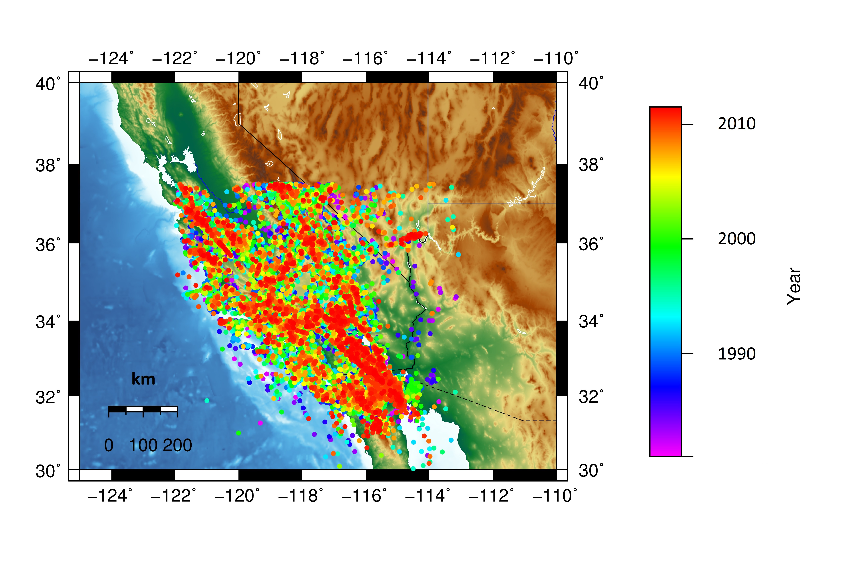
\includegraphics[width=0.95\linewidth]{erdbeben1}
	\label{fig:erdbeben1}
\end{figure}
	\end{frame}
	
		\begin{frame}
		\begin{figure}
			\centering
			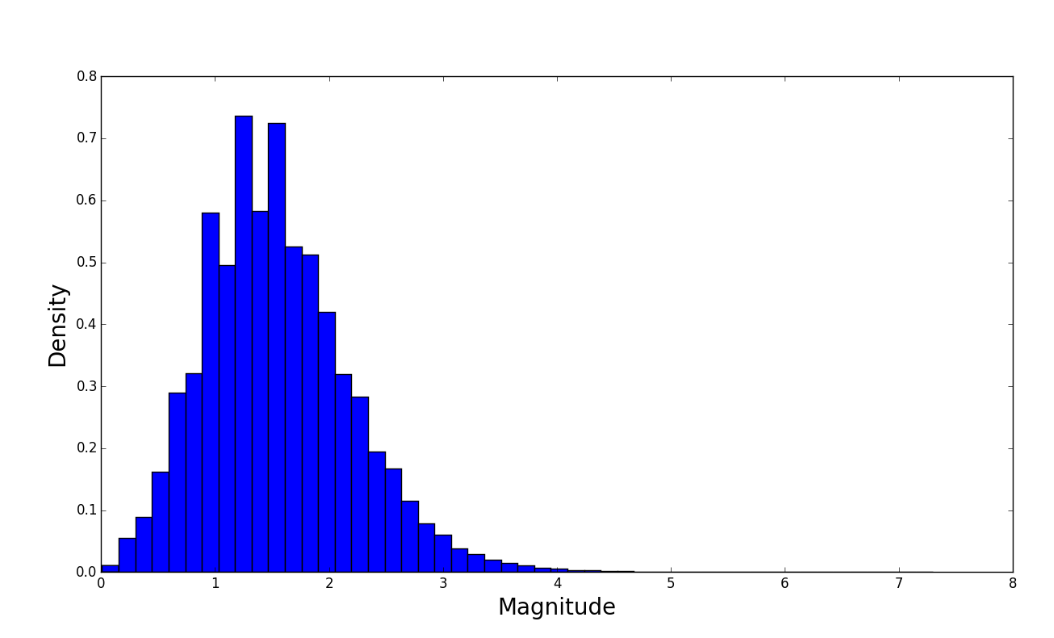
\includegraphics[width=0.95\linewidth]{erdbeben2}
			\label{fig:erdbeben2}
		\end{figure}
	\end{frame}
	
		\begin{frame}
		\begin{figure}
			\centering
			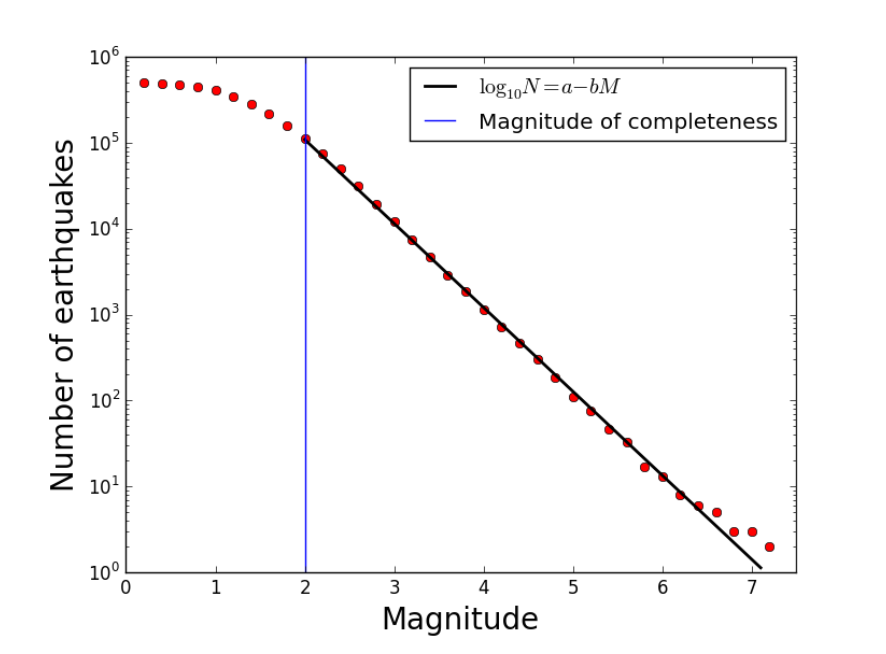
\includegraphics[width=0.95\linewidth]{erdbeben3}
			\label{fig:erdbeben1}
		\end{figure}
	\end{frame}
	
	
	\begin{frame}{Schätzung von $b$ mit Polya-Gamma Data Augmentation}
		\begin{itemize}
			\item Die Bayesianische Schätzung von $b$ kann mit einer Polya-Gamma Data Augmentation erfolgen.
			\item Durch Umformung der Likelihood-Funktion in ein logistisches Modell:
			\begin{equation}
				P(y_i = 1 | m_i, b) = \frac{1}{1 + e^{-m_i b}}
			\end{equation}
			kann die Polya-Gamma-Methode für effizientes Gibbs Sampling genutzt werden.
			\item Dies könnte helfen, robuste Schätzungen für seismische Aktivitätsparameter zu erhalten.
		\end{itemize}
	\end{frame}
	
	
%	\begin{frame}{Das Gutenberg-Richter-Gesetz für Erdbeben}
%		\begin{itemize}
%			\item Das Gutenberg-Richter-Gesetz beschreibt die Häufigkeit von Erdbeben in Abhängigkeit von ihrer Magnitude.
%			\item Es folgt der Beziehung:
%			\begin{equation}
%				\log N(m) = a - b m
%			\end{equation}
%			where:
%			\begin{itemize}
%				\item $N(m)$ die Anzahl der Erdbeben mit einer Magnitude größer als $m$ ist,
%				\item $a$ ein empirischer Parameter ist, der die gesamte seismische Aktivität in einer Region beschreibt (je größer $a$, desto mehr Erdbeben treten auf),
%				\item $b$ die Steigung der Beziehung bestimmt und damit die relative Häufigkeit von großen gegenüber kleinen Erdbeben beschreibt. Typischerweise liegt $b$ zwischen 0,8 und 1,2.
%			\end{itemize}
%		\end{itemize}
%	\end{frame}
	
	\begin{frame}{Schätzung von $b$ mit Polya-Gamma Data Augmentation}
		\begin{itemize}
			\item Die Bayessche Schätzung des Parameters $b$ kann durch eine Polya-Gamma Data Augmentation erleichtert werden.
			\item Durch Umformung der Gutenberg-Richter-Gleichung in ein logistisches Modell:
			\begin{equation}
				P(y_i = 1 | m_i, b) = \frac{1}{1 + e^{-m_i b}}
			\end{equation}
			kann die Polya-Gamma-Methode genutzt werden, um eine Gibbs-Sampling-Strategie zur Bestimmung von $b$ zu entwickeln.
			\item Vorteile dieser Methode:
			\begin{itemize}
				\item Sie ermöglicht eine robuste Schätzung von $b$, selbst bei kleinen oder verrauschten Daten.
				\item Durch die Bayesianische Herangehensweise können Unsicherheiten in der Schätzung direkt quantifiziert werden.
				\item Sie erlaubt eine natürliche Einbindung zusätzlicher a-priori Informationen über $b$.
			\end{itemize}
		\end{itemize}
	\end{frame}
	
	
	\begin{frame}{Warum Polya-Gamma für die Schätzung?}
%		Weglassen??
		\begin{itemize}
			\item Modellierung der Erdbebenhäufigkeit als Poisson-Prozess:
			\[ N(M) \sim \text{Poisson}(\lambda(M)) \]
			\item Log-Transformation führt zu einem linearen Modell:
			\[ \log N(M) = a - bM \]
			\item Durch die Polya-Gamma Methode wird Gibbs-Sampling zur Schätzung ermöglicht.
		\end{itemize}
	\end{frame}
	
	
	
	
	\begin{frame}{Summary}
		\begin{itemize}
			\item Die Polya-Gamma Distribution vereinfacht die Bayessche Inferenz für logistische Modelle erheblich.
			\item Die Gibbs-Sampling-Strategie ermöglicht effiziente numerische Berechnungen.
			\item Die Methode ist gut geeignet für großskalige Datenanalysen und maschinelles Lernen.
		\end{itemize}
	\end{frame}
	




	\begin{frame}{References}
		Polson, N. G., Scott, J. G.,  Windle, J. (2013). Bayesian inference for logistic models using Polya-Gamma latent variables. \textit{Journal of the American Statistical Association}, 108(504), 1339-1349.
	\end{frame}


\begin{frame}{Anhang: Bedeutung der Parameter $b$ und $c$ in der Polya-Gamma Distribution}
	\begin{itemize}
		\item **Parameter $b$ (Shape-Parameter):**
		\begin{itemize}
			\item Gibt an, wie stark die Verteilung skaliert ist.
			\item Höhere Werte machen die Verteilung schmaler und konzentrierter.
			\item Wird oft aus der Anzahl der Trials im Modell abgeleitet.
		\end{itemize}
		\item **Parameter $c$ (Skalenparameter):**
		\begin{itemize}
			\item Steuert die exponentielle Dämpfung.
			\item Höhere Werte von $c$ verschieben die Verteilung nach links.
			\item In logistischen Modellen ist $c = x^T \beta$.
		\end{itemize}
	\end{itemize}
\end{frame}

\begin{frame}{Anhang: Auswirkungen von $b$ und $c$ auf die Verteilung}
	\begin{itemize}
		\item Falls $b = 1$ und $c = 0$: Die Verteilung ähnelt einer Gamma-Verteilung.
		\item Falls $c$ steigt: Die Verteilung wird nach links verschoben.
		\item Falls $b$ steigt: Die Verteilung wird schmaler und konzentrierter.
	\end{itemize}
	\centering
	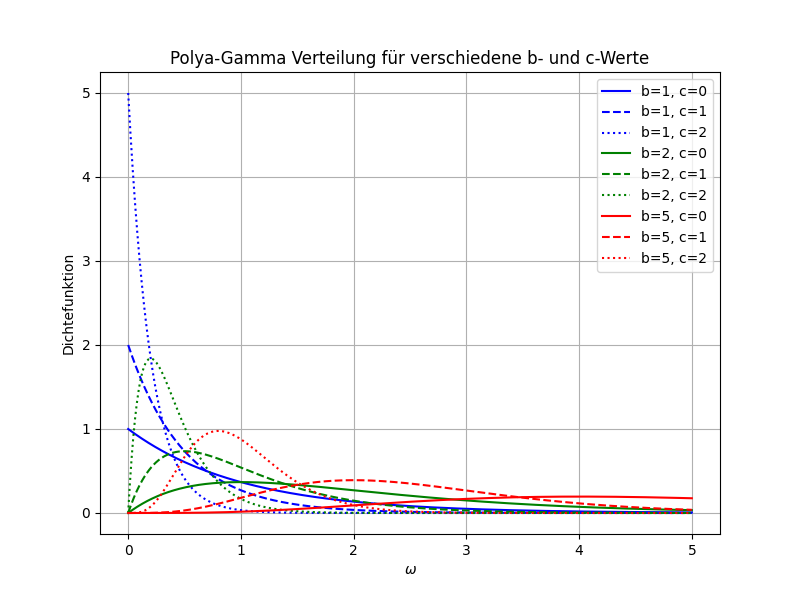
\includegraphics[width=0.6\textwidth]{polya_gamma_distribution.png}
\end{frame}

\begin{frame}{Anhang: Warum ist $p(\omega_i | 1, 0)$ in der Likelihood-Transformation?}
	\begin{itemize}
		\item In der logistischen Regression ergibt sich die Likelihood:
		\begin{equation}
			P(y_i = 1 | x_i, \beta) = \frac{1}{1 + e^{-x_i^T \beta}}
		\end{equation}
		\item Durch die Polya-Gamma-Transformation wird dies umgeschrieben als:
		\begin{equation}
			P(y_i = 1 | x_i, \beta) = \int_0^\infty e^{-\omega_i (x_i^T \beta)^2 / 2} p(\omega_i | 1, 0) d\omega_i
		\end{equation}
		\item **Warum $PG(1,0)$?**
		\begin{itemize}
			\item $b = 1$ weil es sich um eine binäre logistische Regression handelt (Bernoulli-Modell).
			\item $c = 0$ weil keine exponentielle Dämpfung benötigt wird.
		\end{itemize}
	\end{itemize}
\end{frame}
	
	
\end{document}
